
\chapter{Industrielle roboter}

Dette kapittelet består foreløpig i notatform. 

\section{Innledning til Industriroboter}

\textbf{Mål:} Introdusere konseptet av industriroboter og deres rolle i moderne industri.

\textbf{Innhold:}
\begin{itemize}
    \item Definisjon av en industrirobot.
    \item Historisk utvikling og hvordan de har transformert industrien.
    \item Typer industriroboter og deres anvendelsesområder.
\end{itemize}

\subsection{Definisjon av en industrirobot}
En \textbf{industrirobot} er en automatisk styrt, programmerbar, multifunksjonell manipulator designet for å flytte materialer, deler, verktøy eller spesialiserte enheter gjennom varierte programmerte bevegelser for utførelsen av ulike oppgaver. Industriroboter er sentrale i moderne produksjons- og monteringslinjer, der de bidrar til å øke effektiviteten, presisjonen og sikkerheten i industrielle prosesser.

Her er noen nøkkelegenskaper som definerer industriroboter:

\begin{itemize}
    \item \textbf{Programmerbarhet}: Industriroboter kan programmeres til å utføre en rekke oppgaver. Dette inkluderer evnen til å utføre komplekse serier av operasjoner og å kunne reprogrammeres for nye oppgaver, noe som gjør dem ekstremt fleksible i industrielle anvendelser.
    \item \textbf{Automatisering}: De opererer automatisk, utfører oppgaver med minimal eller ingen menneskelig intervensjon etter at de er programmert og satt i drift.
    \item \textbf{Multifunksjonalitet}: De kan utføre et bredt spekter av oppgaver, inkludert, men ikke begrenset til, sveising, maling, montering, plukking og plassering, produktinspeksjon, og pakking. Dette oppnås ofte ved å bytte ut endeffektoren (verktøyet eller griperen) på robotarmen.
    \item \textbf{Nøyaktighet og presisjon}: Industriroboter kan utføre oppgaver med høy grad av nøyaktighet og repeterbarhet, noe som er kritisk i mange produksjonsprosesser.
    \item \textbf{Bevegelseskontroll}: De har avanserte kontrollsystemer som styrer deres bevegelser med stor presisjon. Dette kan inkludere lineære eller roterende bevegelser i flere akser.
\end{itemize}

Industriroboter er en integrert del av den fjerde industrielle revolusjonen (Industri 4.0), der de samhandler med andre digitale systemer og teknologier for å skape smarte og automatiserte produksjonsmiljøer. De bidrar til økt produksjonseffektivitet, forbedret produktkvalitet, reduserte produksjonskostnader, og forbedret arbeidssikkerhet ved å ta over farlige, skitne, eller monotone oppgaver som tidligere ble utført av mennesker.

\subsection{Industrirobotenes Revolusjon: En Titt på Den Historiske Utviklingen og Transformasjonen av Industrien}


\subsubsection{Fra konsept til virkelighet: De tidlige årene}

Reisen begynte på 1950-tallet, et tiår som vitnet om fødselen av den første industriroboten. George Devol, en oppfinner med en fremtidsrettet visjon, skapte Unimate, den første digitale og programmerbare roboten. Med Joseph Engelberger's entreprenørånd, kjent som "robotikkens far", ble Unimate introdusert til verden på 1960-tallet. Denne roboten var designet for å utføre enkle, men farlige oppgaver, som å håndtere varme metaller i støperier, noe som umiddelbart satte standarden for robotteknologiens potensiale i industrielle applikasjoner.

\subsubsection{Ekspansjon og innovasjon: 1970-tallet til 1990-tallet}

Etter introduksjonen av Unimate, så verden en rask utvikling og adopsjon av robotteknologi i ulike sektorer. På 1970-tallet ble robotteknologien mer sofistikert, med introduksjonen av mikroprosessorer som tillot større fleksibilitet og kontroll. Denne perioden så også fremveksten av seksaksede roboter, som tilbød en uovertruffen bevegelsesfrihet og åpnet døren for mer komplekse applikasjoner.

1980- og 1990-tallet var preget av ytterligere innovasjon, hvor roboter ble utstyrt med avansert sensorikk og programvare, som muliggjorde automatisert beslutningstaking og forbedret interaktivitet med menneskelige operatører. Dette la grunnlaget for integrasjonen av roboter i mer finstemte og detaljerte produksjonsprosesser, som elektronikkmontering og bilproduksjon.

\subsubsection{Den fjerde industrielle revolusjonen: 2000-tallet og fremover}

Inngangen til det 21. århundre og fremveksten av Industri 4.0 har markert en ny æra for industriroboter. Med fremveksten av kunstig intelligens (AI), maskinlæring, og Internett-ting (IoT), har industriroboter blitt enda mer intelligente, selvstendige og nettverkskoblede. Denne teknologiske synergien har ført til utviklingen av smarte fabrikker, hvor roboter kommuniserer med hverandre og med produksjonssystemer, for å optimalisere produksjonsflyten og ta autonome beslutninger basert på sanntidsdata.

\subsubsection{Transformasjonen av industrien}

Industrirobotenes evolusjon har fundamentalt transformert produksjonslandskapet. Ved å ta over repetitive, farlige, eller presisjonskrevende oppgaver, har roboter gjort det mulig for industrier å forbedre produktivitet, sikkerhet og produktkvalitet. De har også åpnet for masseproduksjon med tilpassede varianter, som møter den moderne forbrukerens krav til skreddersøm.

Videre har robotteknologi demokratisert produksjonen ved å gjøre avansert produksjonsteknologi tilgjengelig for små og mellomstore bedrifter, noe som fører til en mer inkluderende og konkurransedyktig industriell økonomi.

\subsubsection{Fremtiden}

Mens vi ser fremover, står industrien på terskelen til ytterligere revolusjonerende endringer drevet av robotteknologi. Med stadig forbedringer innen AI og robotikk, kan vi forvente en fremtid hvor roboter ikke bare utfører oppgaver, men også forutser behov og tilpasser seg endrende produksjonsmiljøer dynamisk.

Industrirobotenes historiske utvikling er ikke bare en kronikk over teknologisk fremgang, men et speilbilde av menneskets uendelige streben etter å overskride sine egne grenser. Som vi fortsetter å utforske nye horisonter innen robotteknologi, er det klart at de mest transformative kapitlene ennå ikke er skrevet.



\subsection{Historien om Trallfa Robot}

Trallfa Robot, nå en del av ABB Robotics, spilte en avgjørende rolle i den tidlige utviklingen av industrielle lakeringsroboter. Grunnlagt i Norge, introduserte Trallfa verdens første lakeringsrobot i 1969, en nyskapning som fundamentalt endret industrielle lakeringsprosesser. Denne roboten forbedret ikke bare effektiviteten og kvaliteten på lakkerte overflater, men bidro også til å redusere helse- og sikkerhetsrisikoer for arbeidere.

\subsubsection{Tidlige Begynnelser}

Trallfa's innovasjon begynte på 1960-tallet med utviklingen av den første lakeringsroboten. Denne roboten var designet for å automatisere maling og lakkering, prosesser som tidligere var utført manuelt, ofte under mindre ideelle arbeidsforhold. Ved å innføre automatisering, satte Trallfa standarden for fremtidig utvikling innen industriell lakkering.

\subsubsection{Teknologisk Utvikling og Innovasjon}

Etter den første suksessen fortsatte Trallfa å utvikle og forbedre sine robotteknologier. Gjennom innovasjon og engasjement for kvalitet, utvidet selskapet funksjonaliteten og anvendeligheten av sine roboter, noe som gjorde dem til et foretrukket valg i mange industrielle applikasjoner.

\subsubsection{Oppkjøpet av ABB}

I 1992 ble Trallfa en del av ABB, en global leder innen kraft og automatiseringsteknologier. Som en del av ABB Robotics, har Trallfa-merkevaren fortsatt å være i forkant av innovasjon, og bidrar til å utvikle avanserte lakeringsroboter som møter dagens industrielle behov.

\subsubsection{Bidrag til Industrien}

Gjennom sin historie har Trallfa Robot, og senere ABB Robotics, bidratt til å transformere lakeringsprosesser. Ved å tilby løsninger som forbedrer produksjonseffektiviteten, produktkvaliteten og arbeidsmiljøet, har de spilt en nøkkelrolle i å gjøre industrien mer bærekraftig og kostnadseffektiv.

\subsubsection{Fremtiden}

Med stadig ny teknologi og innovasjon ser fremtiden for industrielle lakeringsroboter lys ut. Trallfa Robot, under ABB Robotics, fortsetter å utforske nye grenser for automatisering, og setter standarden for neste generasjons industrielle lakeringsløsninger.


\subsection{Typer av Industriroboter og Deres Anvendelsesområder}

\subsubsection{Artikulerte Robotarm}

Artikulerte robotarmer har roterende ledd med to til ti eller flere akser, som gir dem en menneskelignende fleksibilitet. De brukes i et bredt spekter av applikasjoner, inkludert sveising, montering, maskinbetjening, maling, og plukk-og-plass-oppgaver.

\subsubsection{SCARA Robot (Selective Compliance Assembly Robot Arm)}

SCARA-roboter er designet for høy-hastighets plukk-og-plass-oppgaver og montering, med 4 akser for rigide vertikale bevegelser og fleksible horisontale bevegelser. De er ideelle for presisjonsmontering, produkttesting, og pakking i elektronikk-, forbrukervarer-, og bilindustrien.

\subsubsection{Kartesiske Roboter / Gantry Roboter}

Disse robotene opererer langs tre ortogonale akser (X, Y, Z) og er kjent for sitt rektangulære arbeidsområde, som dekker store områder og bærer tunge laster. Anvendelsesområder inkluderer CNC-maskinbetjening, 3D-printing, pallisering, og materialhåndtering.

\subsubsection{Delta Roboter}

Kjent for sin spindelvev-lignende struktur og raske bevegelser, brukes Delta-roboter ofte i høyhastighets plukk-og-plass-oppgaver, spesielt i næringsmiddelindustrien, pakking, og sortering.

\subsubsection{Sylinderrobotter}

Sylinderroboter har en sylindrisk arbeidsområde og opererer innenfor et sylindrisk koordinatsystem, som gir dem et unikt bevegelsesmønster. De er godt egnet for enkle monteringsoppgaver, materialhåndtering, og plukk-og-plass-applikasjoner.

\subsubsection{Parallell Roboter}

Også kjent som parallellkinematiske maskiner, disse robotene har armer med stive sammenkoblinger som beveger seg parallelt med hverandre. De brukes i applikasjoner som krever høy presisjon og hastighet.

\subsubsection{Samarbeidende Roboter (Cobots)}

Cobots er designet for å jobbe sammen med mennesker i en delt arbeidsprosess, utstyrt med sensorer og programvare for å sikre sikker interaksjon. De anvendes i et bredt spekter av sektorer for oppgaver som kan utføres side om side med menneskelige arbeidere.




\section{Teknologi og Operasjon}

\textbf{Mål:} Forstå teknologiene som driver industriroboter og grunnleggende om hvordan de opererer.

\textbf{Innhold:}
\begin{itemize}
    \item Oversikt over mekanisk design og kinematikk.
    \item Introduksjon til robotstyringssystemer og programvare.
    \item Sensorer og aktuatorer som brukes i industriroboter.
    \item Sikkerhetsstandarder og -protokoller for drift.
\end{itemize}

\section{Programmering av Industriroboter}

\textbf{Mål:} Lære grunnleggende prinsipper for programmering av industriroboter.

\textbf{Innhold:}
\begin{itemize}
    \item Introduksjon til robotprogrammeringsspråk.
    \item Enkel programmeringsøvelse (f.eks., å programmere en robotarm til å utføre en enkel oppgave).
    \item Bruk av simuleringsprogramvare for å teste robotprogrammer.
\end{itemize}

\section{Anvendelser av Industriroboter}

\textbf{Mål:} Utforske hvordan industriroboter brukes i ulike sektorer.

\textbf{Innhold:}
\begin{itemize}
    \item Case-studier av robotanvendelse i bilindustrien, elektronikk, matvareproduksjon, og mer.
    \item Diskusjon om roboters rolle i automatisering og effektivisering av produksjonsprosesser.
    \item Fremtidens trender innen robotteknologi og nye anvendelsesområder.
\end{itemize}

\section{Industriroboter og Samfunnet}

\textbf{Mål:} Reflektere over innvirkningen av industriroboter på arbeidsmarkedet og samfunnet.

\textbf{Innhold:}
\begin{itemize}
    \item Debatt om automatiseringens effekt på arbeidsplasser.
    \item Diskusjon om etikk rundt bruk av roboter (f.eks., beslutningstaking utført av maskiner).
    \item Hvordan utdanning og ferdigheter må tilpasse seg den økende bruken av robotteknologi.
\end{itemize}

\section{Praktisk Øvelse og Prosjektarbeid}

\textbf{Mål:} Anvende teoretisk kunnskap i praktisk arbeid.

\textbf{Innhold:}
\begin{itemize}
    \item Gruppeprosjekt hvor studentene designer en løsning med bruk av industriroboter for en gitt industriell prosess.
    \item Presentasjon og diskusjon av prosjektarbeidet.
\end{itemize}

\section{Avslutning og Evaluering}

\textbf{Mål:} Oppsummere læringsutbyttet og evaluere kursopplegget.



$$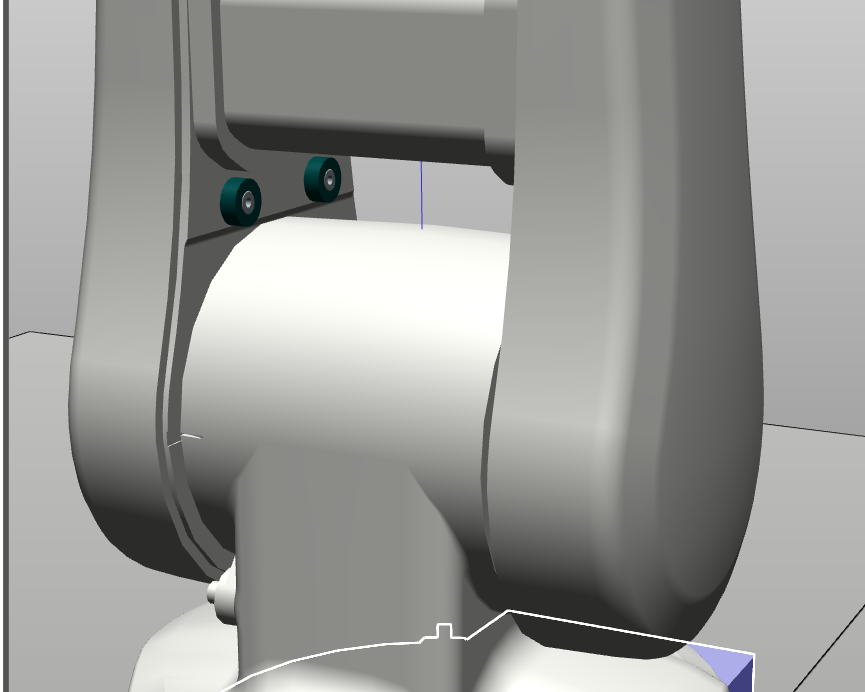
\includegraphics[width=16cm]{./Robot01.png}$$
\section{trandisjonelle roboter}

Insustrielle roboer har ofte en struktur som en mennesklig arm.

\begin{itemize}%%[noitemsep]
\item opp til  6 akser
\item plukk og plaser syklus på 300-500ms med deler på et par kg. 
\item Sveiseroboter
\end{itemize}


Hva kjennetegner en industriell robot:
\begin{itemize}%[noitemsep]
\item den kjører automatisk
\item den kan reprogrammeres
\item den har en arm med mer en tre akser som en kan feste ulike verktøy på
\item den kan enten stå fast eller være flyttbare
\item den er laget for å løse industrelle oppgaver 
\end{itemize}

Ulike industrielle roboter kan være:
\begin{itemize}%[noitemsep]
\item Linære roboter
\item SCARA roboter
\item Parallelle roboter
\item Artikulerte roboter
\item Sylindriske roboter
\end{itemize}

Eksempler på industrielle bruksområder:


\begin{itemize}%[noitemsep]
\item Forflytting av metall i deleproduksjon eller støyping
\item palletering
\item sveising
\item lakkering
\item pakking
\item automatisk lagersystem
\end{itemize}



Mekanisk teori:
\begin{itemize}%[noitemsep]
\item mekanismer og grader av frihet
\item kinematikk?
\item Arbeidsområde og leddområde
\item redundans og singularitet
\end{itemize}

Styring:
\begin{itemize}%[noitemsep]
\item bane planlegging
\item posisjon, kraft og impedanse kontrol
\item læring av baner
\end{itemize}



Robotsystemer:
\begin{itemize}%[noitemsep]
\item Robots functional schematics
\item End-effectors and tools
\end{itemize}







%%%%%%%%%%%%%%%%%%%%%%%%%%%%%%%%%%%%%%%%%%%%%%%%%%%%

